

\documentclass{beamer}

\mode<presentation> {

% The Beamer class comes with a number of default slide themes
% which change the colors and layouts of slides. Below this is a list
% of all the themes, uncomment each in turn to see what they look like.


\usetheme{Boadilla}



\setbeamertemplate{footline}  


}
\setbeamersize{text margin left=1cm, }
\setbeamertemplate{frametitle}[default][center]
\usepackage{graphicx} 
\usepackage{booktabs} 

	\usepackage{changepage}


\usepackage{cite}
\usepackage{setspace}
\usepackage{color}
\usepackage[normalem]{ulem}
\newtheorem{hyp}{Hypothesis}


\usepackage{epsfig}
\usepackage{amsmath}
\usepackage{amssymb}
\usepackage{multicol}
\usepackage{amsmath, amsthm, amssymb}


\usepackage{graphicx}
\usepackage{tikz}
\usetikzlibrary{shapes,arrows}
\usepackage{tikz}
\usepackage{amsmath, amsthm, amssymb}
%----------------------------------------------------------------------------------------
%	TITLE PAGE
%----------------------------------------------------------------------------------------



\begin{document}
	

  

\begin{frame}
	\frametitle{Introduction to Data Science}
	\pause 
	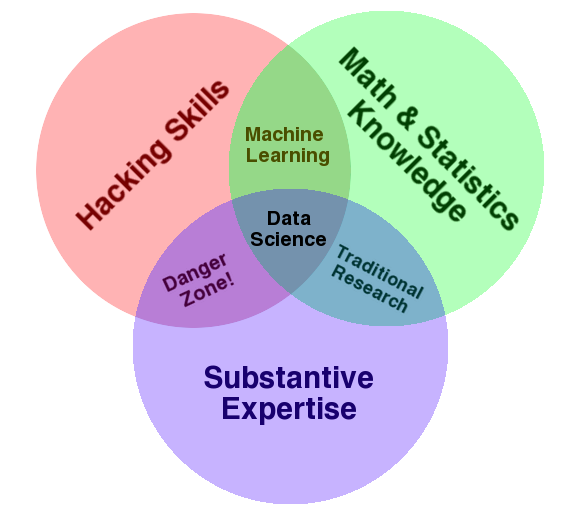
\includegraphics[ scale=.45]{figures/conway_venn.png} \\
\end{frame}




\begin{frame}
	
	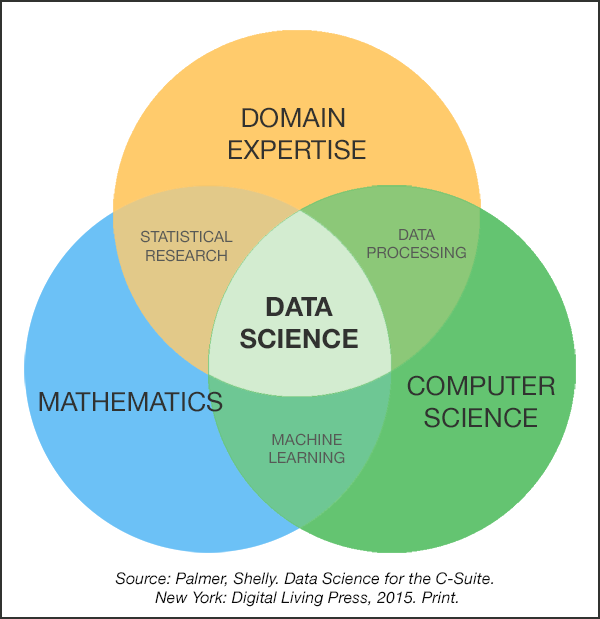
\includegraphics[ scale=.3]{figures/fancy_venn.png} \\
	
\end{frame}


\begin{frame}
	
	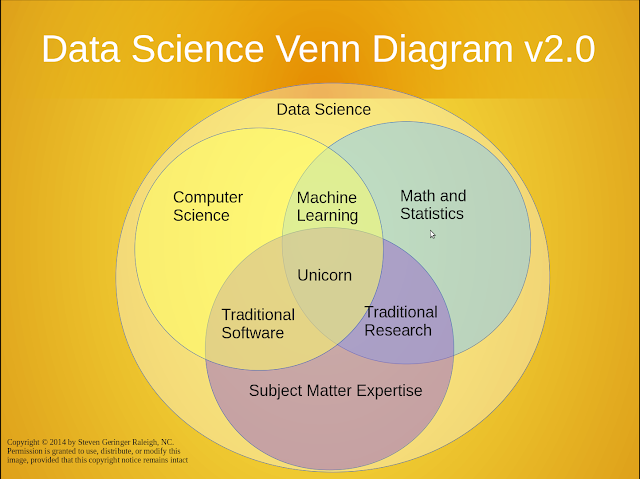
\includegraphics[ scale=.5]{figures/nice_venn.png} \\
	
	
	
\end{frame}	

\begin{frame}
	
	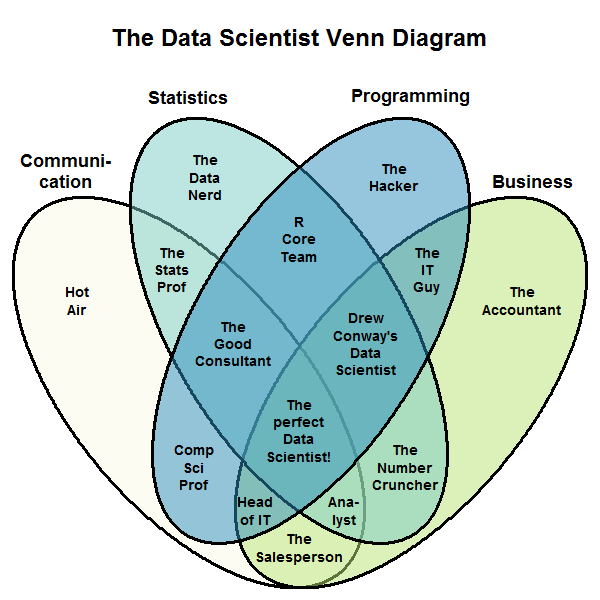
\includegraphics[ scale=.4]{figures/many_bubbles_venn.png} \\
	
	
	
\end{frame}	


\begin{frame}
	
	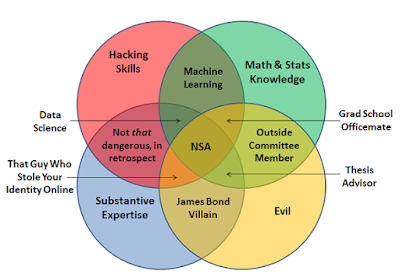
\includegraphics[ scale=.7]{figures/danger_venn.png} \\
	
	
	
\end{frame}	
	
	
\begin{frame}
	
	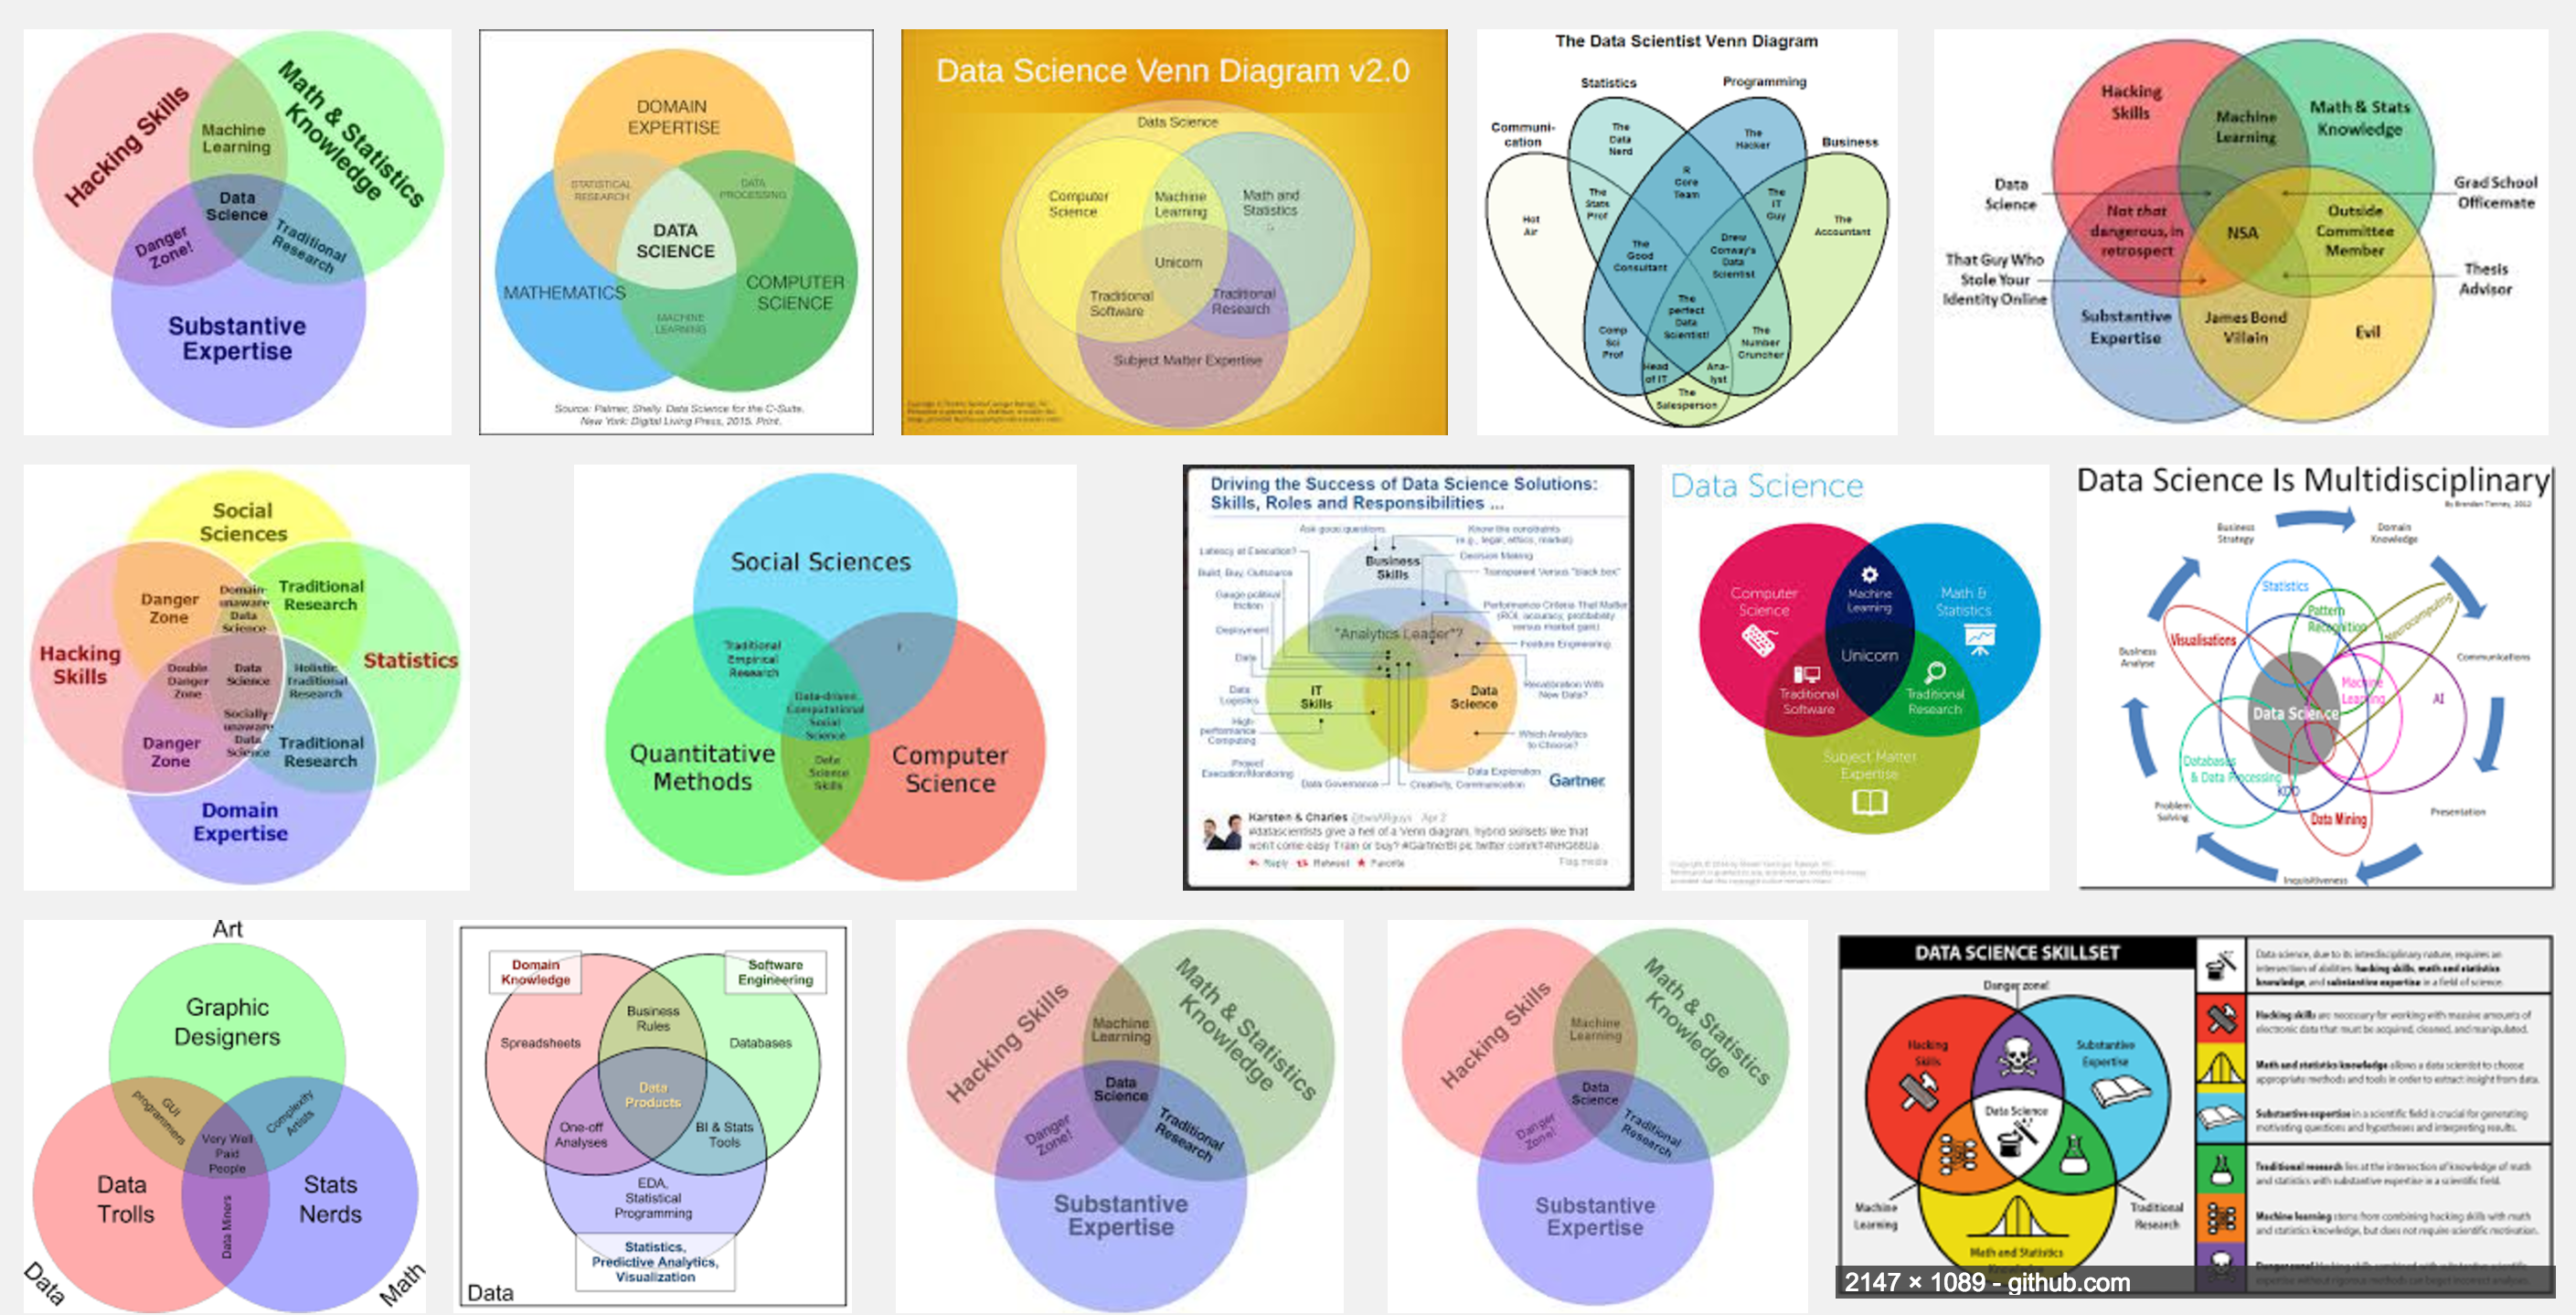
\includegraphics[ scale=.2]{figures/meta_venn.png} \\
	
	
	
\end{frame}		
	
%%%%%%%%%%%%%%%%%%%%%%%%%%%
\begin{frame}
	
	\begin{center}
		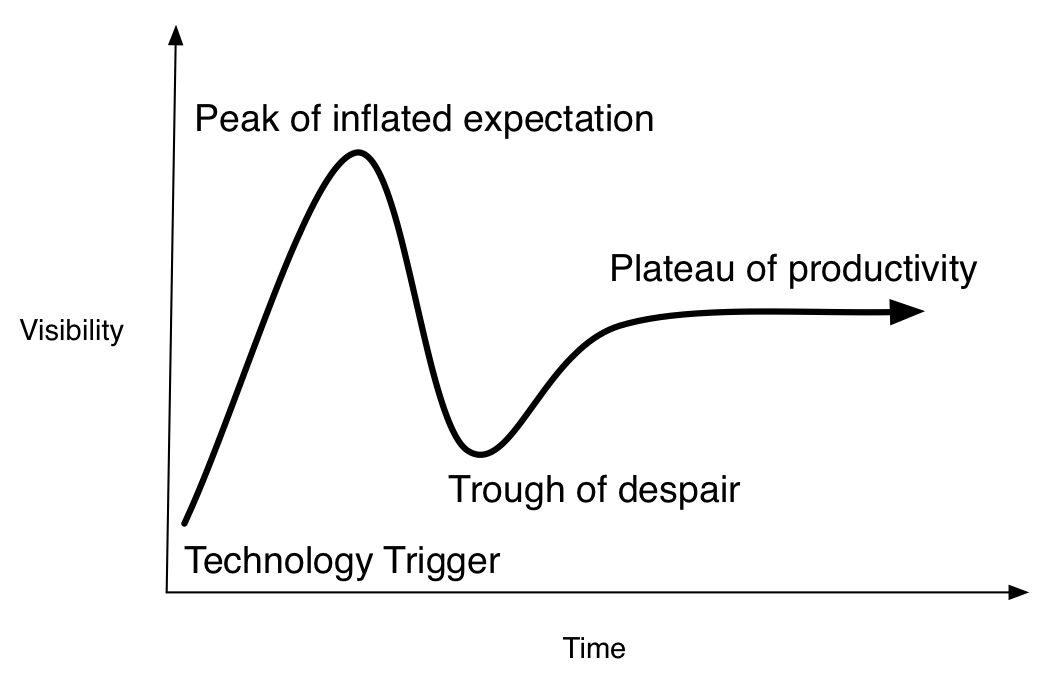
\includegraphics[width=\textwidth]{figures/hype_cycle}
	\end{center}
	
	
	\Tiny{\url{https://commons.wikimedia.org/wiki/File:Gartner_Hype_Cycle.svg}}
	
\end{frame}
%%%%%%%%%%%%%%%%%%%%%%%%%%%	

\begin{frame}
	\frametitle{About Me}
	\begin{itemize}
		
		\item PhD in Political Science from NYU
		\pause
		\vspace{1em}
		\item 4 semesters TA'ing in NYU's Masters in Data Science; 3 of those Intro to DS
		\pause
		\vspace{1em}
		\item Starting as Assistant Professor of Political Science at Penn State in the Fall
		\pause
		\vspace{1em}
		\item Research interests
		
		\pause
\begin{itemize}
	\item Social Media
	\pause 
	\item Text as Data
	\pause 
	\item Online harassment/hate speech
	\pause
	\item Political polarization
\end{itemize}

		
	\end{itemize}
\end{frame}
	
	



\begin{frame}
	\frametitle{My Research}
	\begin{itemize}
		
		\item Sample of white men (or fully anonymous users) harassing others using racial slur
		\pause 
		\begin{figure}
			
			
			
\includegraphics[scale=.10]{figures/white_black_bot_comparison.png}
		\end{figure}
		\pause
		\item ``[@subject] Hey man, just remember that there are real people whose feelings are hurt when you use that kind of language"
		\pause
		\item White, high-status bot (sock puppet) caused subjects to tweet fewer racial slurs
		\pause
		\item Reactance: black, low-status bot caused subjects to tweet \textit{more} racial slurs
		\pause
		\item Social identity and status affect the enforcement of behavioral norms
		
		
	\end{itemize}
\end{frame}	
	



\begin{frame}
	\frametitle{My Research}
	\begin{itemize}
		
		
		

			\item 2014 Protests in Venezuela 


			\begin{itemize}
				\item We analyze elite Twitter use \pause
				\item Regime and opposition elites are quantitatively similar prior  \pause

				\item The opposition elites keep talking about the protests, while the regime tries to advance various other narratives, to distract from the protests \pause

				
			\end{itemize}


		
	\end{itemize}
\end{frame}	


\begin{frame}
	\frametitle{My Research}
		
		\begin{figure}
			
			
			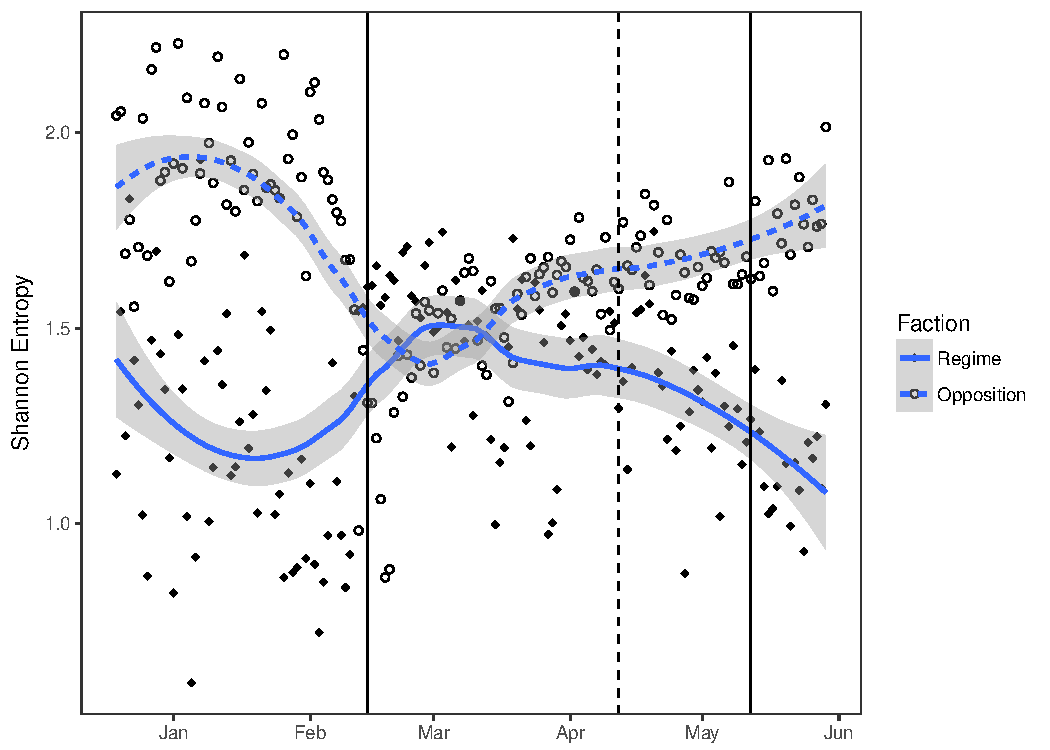
\includegraphics[scale=.5]{figures/fig3.pdf} \\
			\raggedright{\small{Each point represents the Topic Diversity score for the opposition and regime tweets respectively, compuated based on their tweets. The vertical lines correspond to the murder of Miss Venezuela, the arrest of L\'{o}pez, and Beginning of the Independence Movement Day, respectively. }}
			
		\end{figure}
\end{frame}	






\begin{frame}
	\frametitle{Overview of the Course}
	
	\href{https://github.com/kmunger/Intro\_Data\_Science\_Rosario}{Course Website}\\ \pause 
	
	\href{https://github.com/kmunger/Intro_Data_Science_Rosario/blob/master/syllabus.pdf}{Syllabus}\\
	
	Much of this course is a combination of courses I have helped teach in the past; all of the materials here are free for anyone to use.
\end{frame}	



\begin{frame}
	\frametitle{Data Science Questions}
	
\begin{itemize}
	\item Will customer X default on her loan? \pause
	

	\item Who might be good ``friends" on our social networking site? \pause
	\item Did X cause Y to happen? \pause 

\item 	Do politicians fall into unique groups? \pause 


\item 	Who wrote this mystery text?
	
\end{itemize}
\end{frame}	



\begin{frame}
	\frametitle{Data}
	
	\begin{itemize}
		\item Found Data v Created Data \pause
		\item Readymades and Custommades
		

		
	\end{itemize}
\end{frame}	



\begin{frame}
	
	\begin{center}
		\begin{tabular}{ccc}
			\onslide<1-3>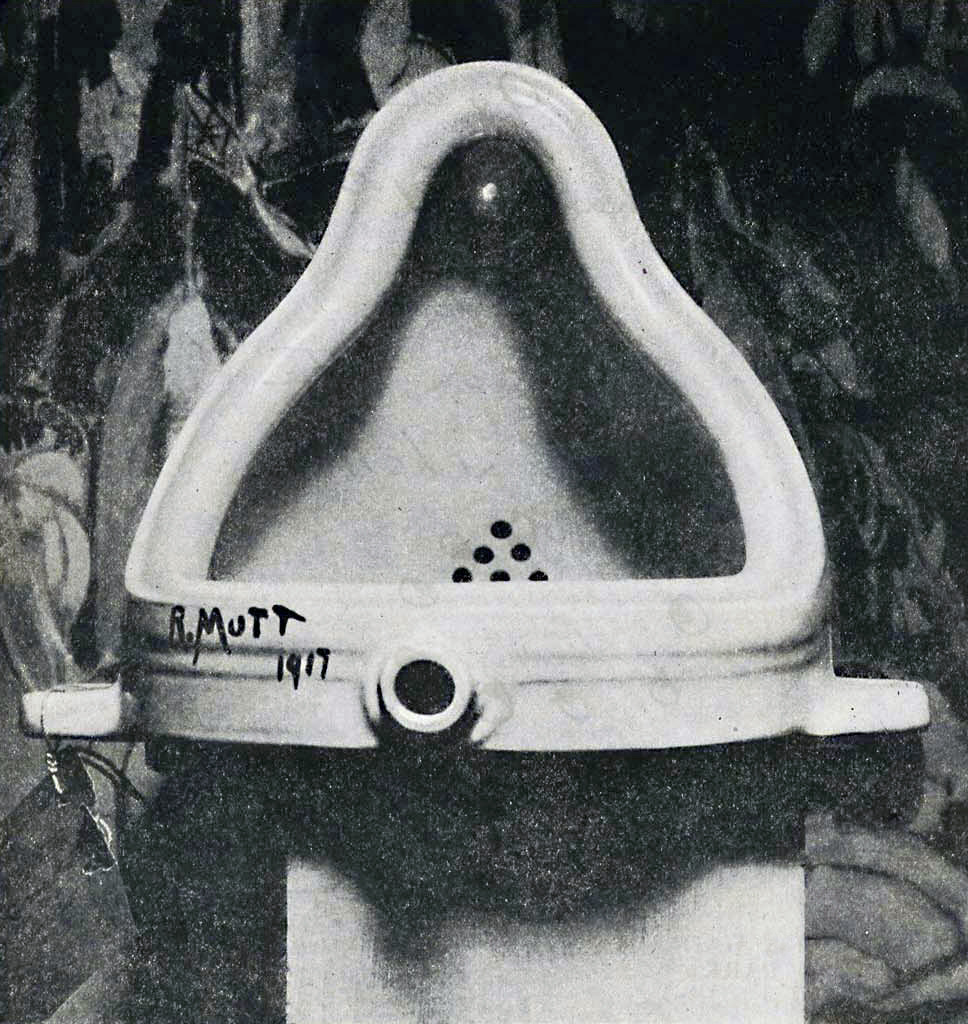
\includegraphics[width=0.30\textwidth]{figures/duchamp_fountain} & \phantom{12345} & \onslide<2-3>{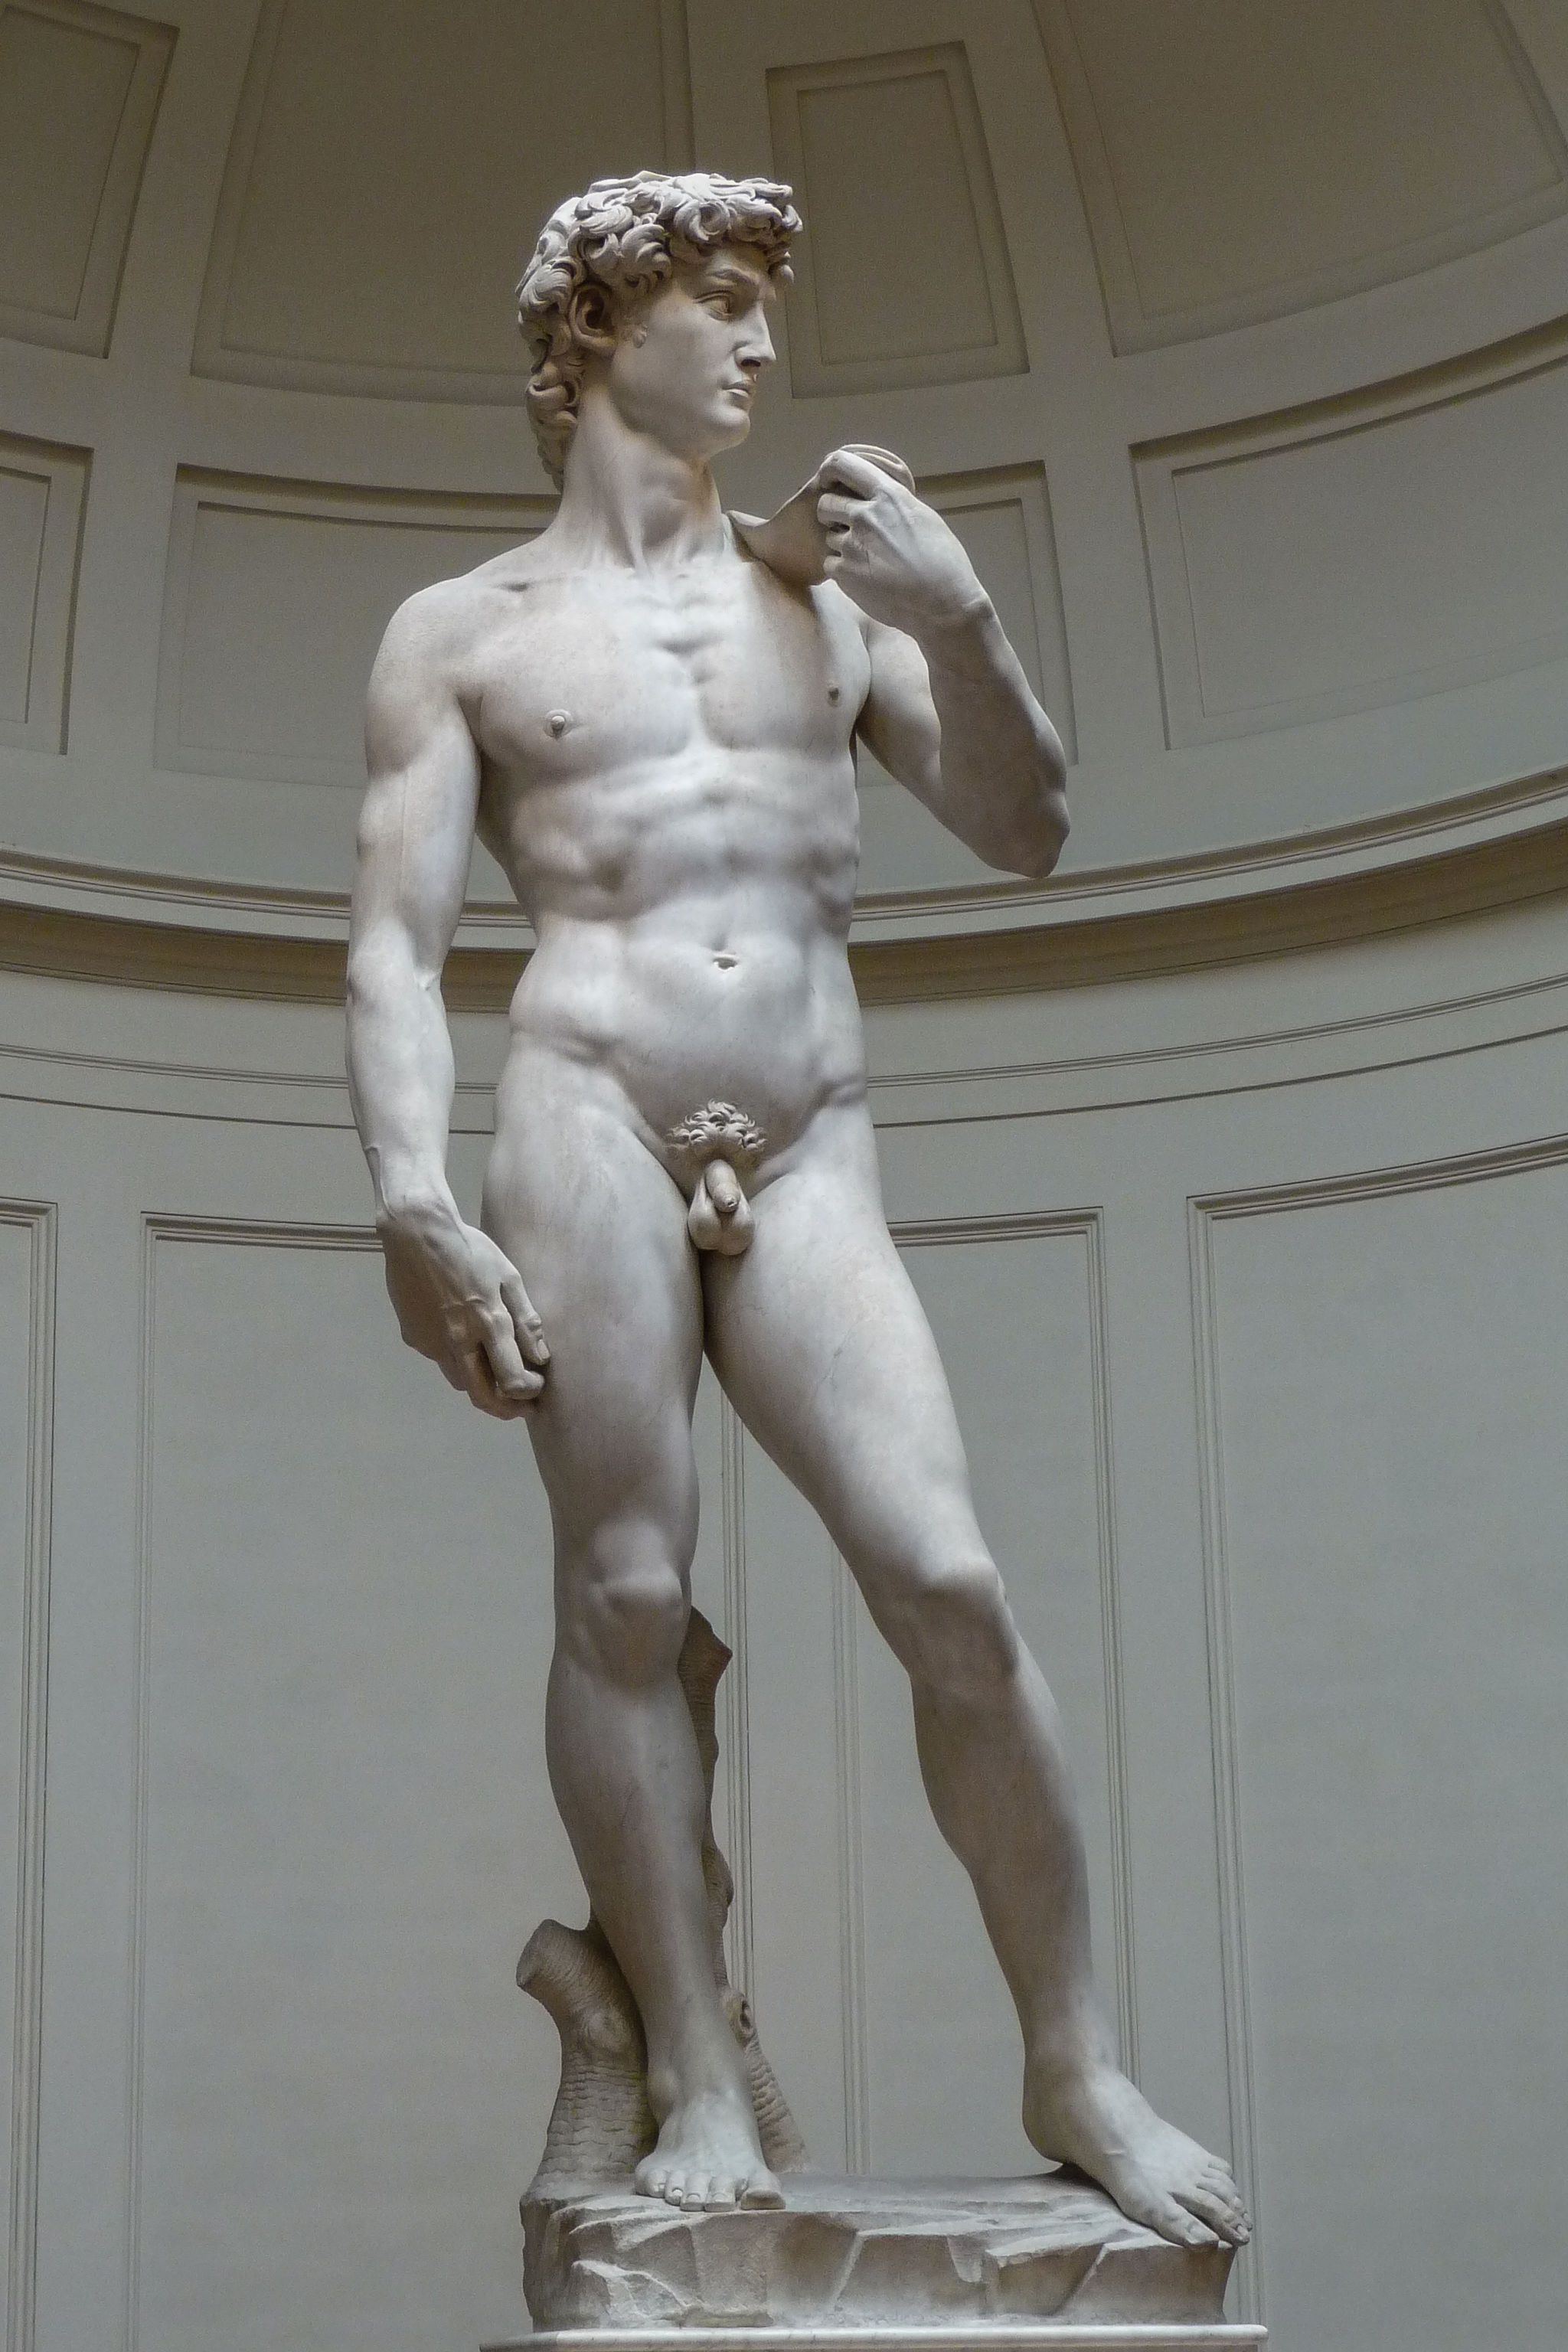
\includegraphics[width=0.30\textwidth]{figures/michelangelo_david}} \\
			\onslide<3>{\LARGE{Readymades}} &  & \onslide<3>{\LARGE{Custommades}}
		\end{tabular}
	\end{center}
	
	
	\vspace{0.5in}
	\onslide<3>{
		\TINY{\url{https://commons.wikimedia.org/wiki/File:Duchamp_Fountaine.jpg}}\\
		\TINY{\url{https://commons.wikimedia.org/wiki/File:\%27David\%27_by_Michelangelo_JBU0001.JPG}}}
	
\end{frame}


\begin{frame}
	\frametitle{Data Science Workflow}
	
	\begin{itemize}
		\item Asking a Question\pause
		\item Data Understanding \pause
		\item Data Manipulation \pause		
		\item Modeling  \pause		
		\item Evaluation  \pause
		\item Implementation/Inference  \pause						
	\end{itemize}
\end{frame}	

\begin{frame}
	\frametitle{Ethics}
	
	\begin{itemize}
		\item Brave new world of data\pause
		\item Rules are not fully understood yet, but the stakes are high \pause
		\item Algorithmic bias \pause 
		\begin{itemize}
			\item Plagiarism software is better at detecting copied text by non-native English speakers \pause 
			\item NYT: ``a Google Images search for `C.E.O' produced 11 percent women, even though 27 percent of United States chief executives are women. (On a recent search, the first picture of a woman to appear, on the second page, was the C.E.O. Barbie doll.)" \pause
		\end{itemize}		
		\item Tendency to re-enforce existing inequalities when using biased data			
	\end{itemize}
\end{frame}	

\begin{frame}
	
	\begin{center}

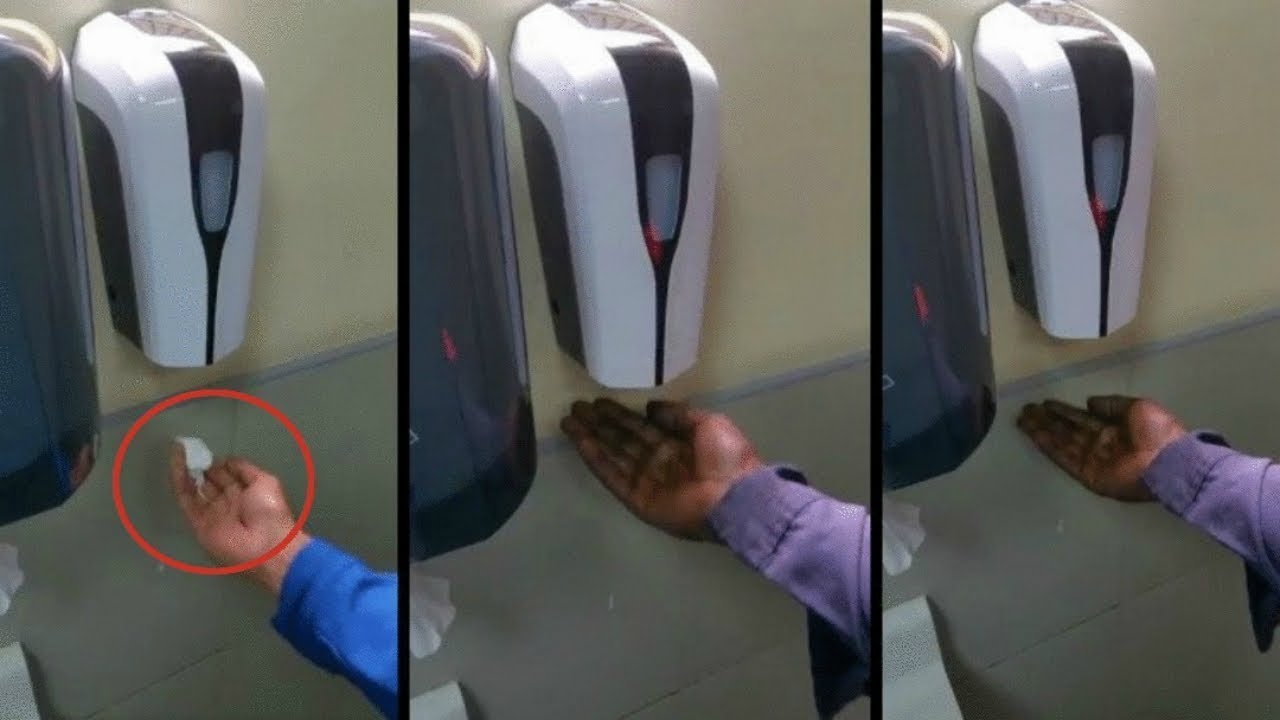
\includegraphics[scale=.2]{figures/racist_soap.jpg}
	\end{center}
	




		\TINY{\url{https://www.youtube.com/watch?v=YJjv_OeiHmo}}
	
\end{frame}

\begin{frame}
	\frametitle{Know Your Data}
	

		 [Example taken from Brian D'Alessandro's NYU course]\\
	

					

	
		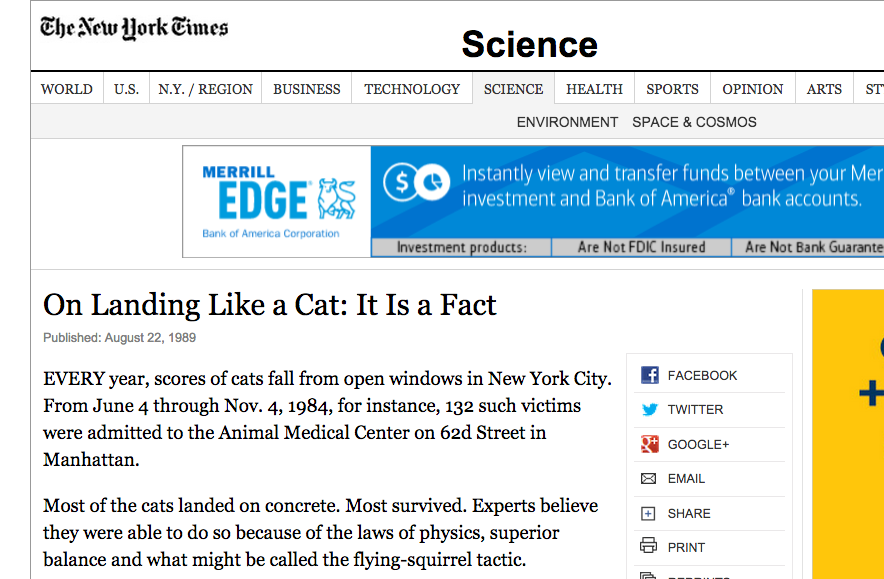
\includegraphics[scale=.34]{figures/nyt_cats.png}\end{frame}




\begin{frame}
	\frametitle{Know Your Data}
	

	
	
	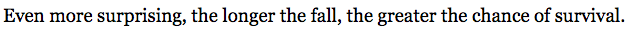
\includegraphics[scale=.5]{figures/nyt_cats_1.png}\\
	
	
		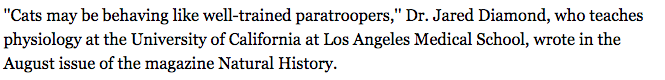
\includegraphics[scale=.5]{figures/nyt_cats_2.png}\\
		\pause
		Selection Bias!
	
	\end{frame}



\begin{frame}
	\frametitle{Survisorship Bias}
	
		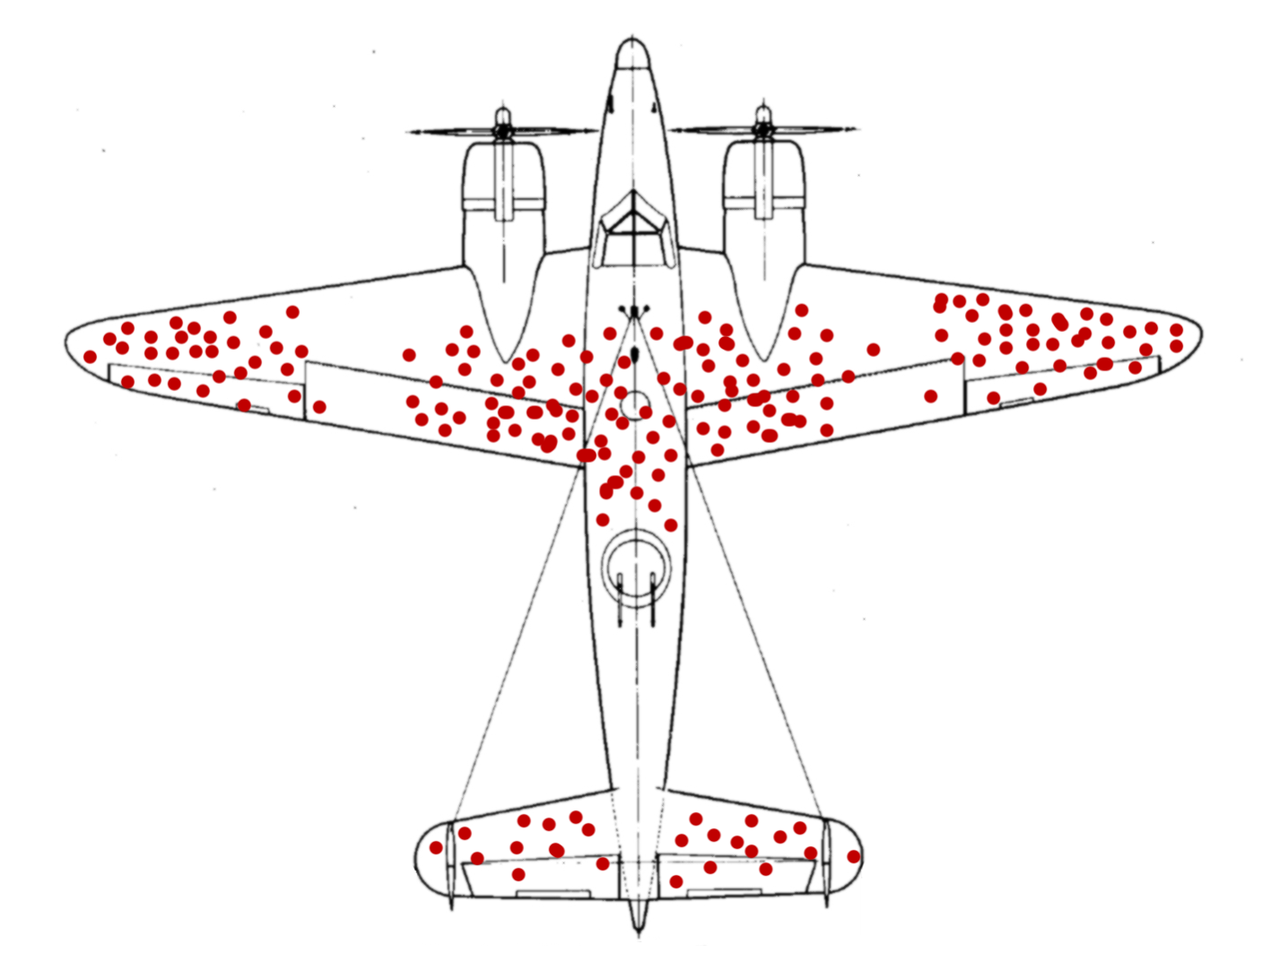
\includegraphics[scale=.25]{figures/airplane.png}\\	

	
\end{frame}

\begin{frame}
	\frametitle{Biased Training Data}
		
		\begin{center}
			
			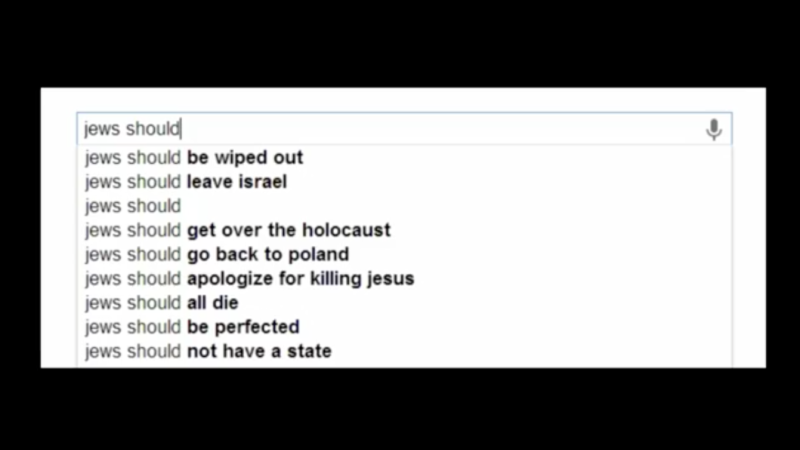
\includegraphics[scale=.7]{figures/biased_google.png}
		\end{center}
		
		
		
		
		
		\TINY{Kate Crawford’s “The Trouble With Bias” at NIPS 2017}
	
\end{frame}



\end{document} 